\documentclass[../main.tex]{subfiles}

\begin{document}
\section{Independent Observations (0D fields)}


\subsection{Univariate Observations}

The bar graph is arguably the simplest way to visualize data that is all of the
same type drawn from a sample at random. In this visualization technique, the
heights of the bar are representative of the values, the x values are each
invidual observation and the positioning of the x values is somewhat
arbitrary. \cite{TufteVisualDIsplay, Friendly, Playfair}. Since bar
graphs become somewhat useless as the number of samples increase, it is common
to group (bin) the data and then count the number of elements in each
been. Both this binning and counting and the subsequent bar chart of the
frequency are referred to as histograms \cite{ioannidis2003}. While histograms
give an approximation of the distribution of the data, sometimes the bin widths
can be too wide and thereby fail to catch naunces in the data such as
bimodality. A way to counteract this is to build histograms with very thin
buckets, which is one of the less sophisticated methods of doing kernal density
estimation. Other methods of approximating the distribution include nearest
neighbor estimation or the  moving windowed average density trace method \cite{chambers1983}.


\subsection{Bivariate Observations}

While bar graphs and histograms start giving a sense of the variability in
data, they are limited to showing the dispersion of the data only in 1
dimension; namely the measurements themselves. In their survey of the history
of the boxplot \cite{wickham2011} Wickham and Stryjewski trace the evolution of
the boxplot from definitive boxes to amorphous envelopes.  They start by laying
out the core statistics of a boxplot, which can also be seen in Figure~\ref{fig:boxplot}.
\begin{description}

\item[Median (Q2)] 50\% quartile
\item[Inter Quartile Range (IQR)]
\end{description}

\begin{tabular}{|r| r |r|r|}
  & Lower & Upper\\
  \multicolumn{2}{Hinge} & Q1: 25\%  & Q3: 75\% \\
  \multicolumn{2}{Interquartile range} & \multicolumn{2}{IQR = Q3-Q1}\\
  \multirow{2}{Fence} & Inner & Q1-1.5*IQR & Q3-1.5*IQR \\
  & outer & Q1-3*IQR & Q3+3*IQR \\
  \end{tabular}

\begin{figure}
  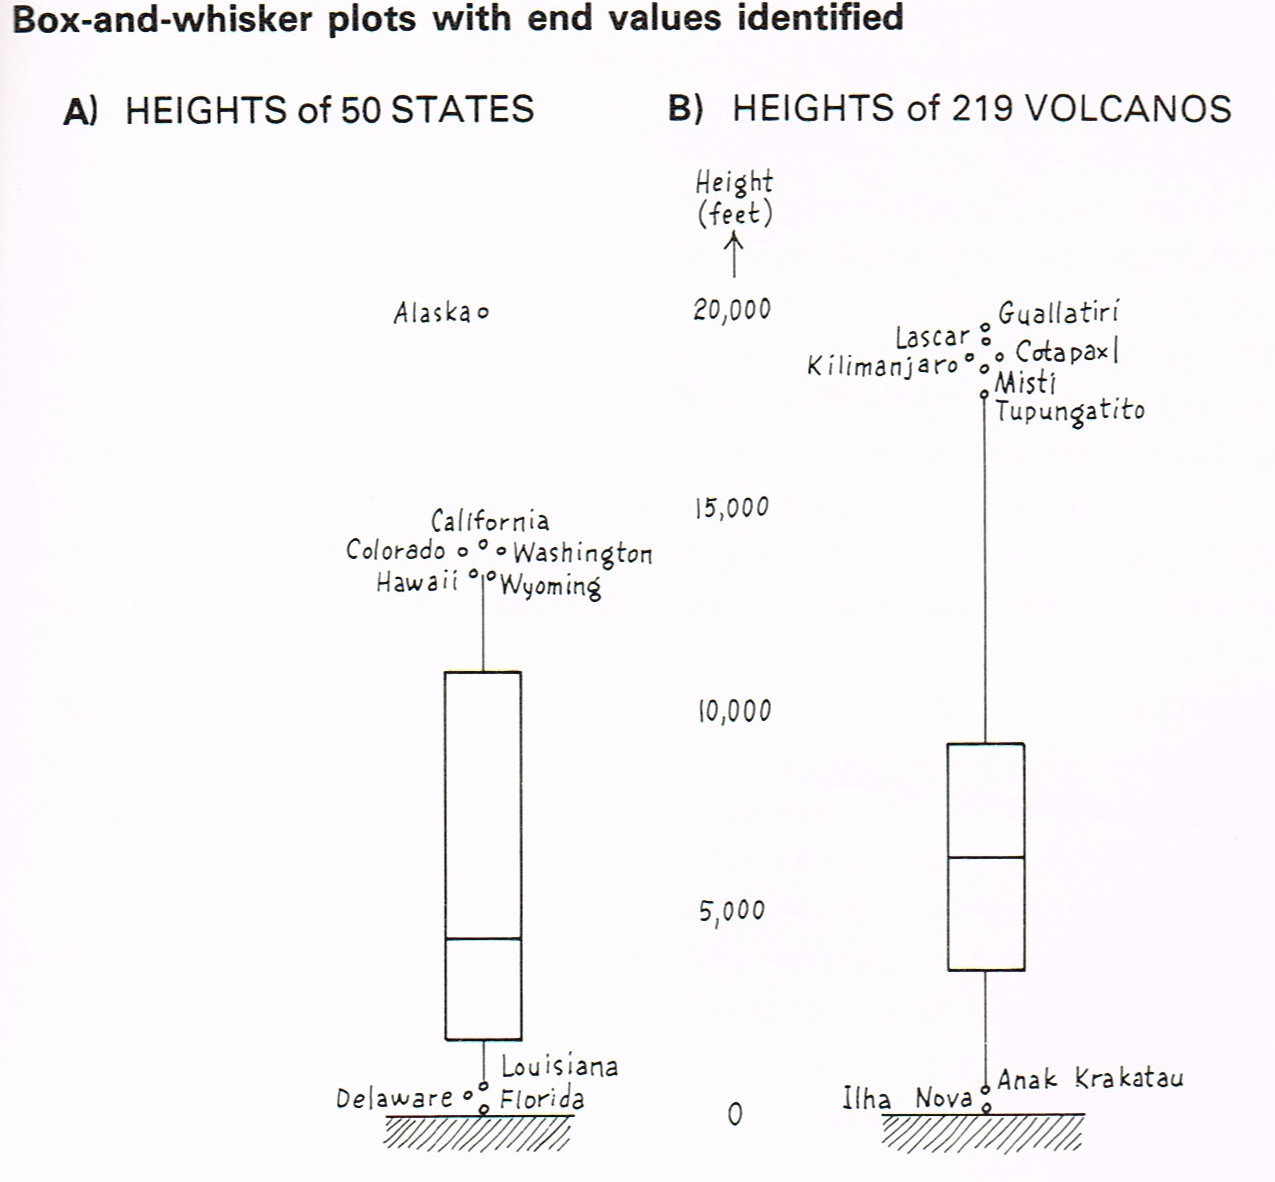
\includegraphics{boxplot}
  \caption{Tukey's 1977 example of the box plot (exhibit 6 of chapter 2 from
    Exploratory Data Analytics\cite{tukey1977}) illustrates how the box plot
    shows
    the distribution of topology of states and
    the distribution of volcanos. The strength of the box and whisker is that
    the
    reader can quickly compare the two distributions and learn, for example,
    that
    volcanos tend to span a shorter range of average heights, but that the
    extremes
    are much further from the center. Essentially, the distributions act as
    references for the other displayed distributions.}
  \label{fig:boxplot}
\end{figure}

In Tukey's introduction to the boxplot \cite{tukey1977}, shown in
Figure~\ref{fig:boxplot}, the box and whisker plot takes the distributional
information of a h\
istogram and encodes the state heights between the
25th and 75th percentiles as a box, the median height as a line cutting across
the heights, and the extreme state heights as lines coming out of the
boxes. While a histogram would also show that the distribution of state heights
has a fat right tail,
the power of the box and whisker plot is in encoding this information such that
it's trivial to compare to it's neighboring distribution of volcano
heights because they can share the Y axis. As the number of distributions grow,
this technique becomes invaluable because the number of histograms that can be
placed next to each other or overlayed as pdfs can quickly become
unweildy.  Many others authors have kept the basic structure of the boxplot,
but exploited the structure to convey more information about the data. Authors
used different quantile levels \cite{hyndman1996}s or measures of outliers
\cite{frigge1989}, or ways of identifying outliers\cite{carter2009,
  schwertman2004, schwertman\
  2007}, or otherwise incorporated skewness,
kurtosis, and other descriptive distributional statistics \cite{kim2004,
  hubert2008, marmolejo\
  2015}.


\subsubsection{Dependent variables}
%%scatter segue into bagplot and HDR?
Arguably the simplest and most well known method of visualizing two
variables against each other is the scatterplot\cite{friendly2005}. In
a scatter plot, one variable is mapped to the x coordinate and a
second variable is mapped to the y coordinate, and the distribution of the
points in the x/y plane indicates whether the x and y variables are related to
each other. While this plot gives a sense of direction, it can fail for larger
datesets (% insert citations for scatter for larger datasets) and doesn't
capture the uncertainity of the relationship between the x and y variables. To
display the distributional variance, the bagplot and bivariate HDR plot were
created. These plots work in X/Y/Z - bag/box papers tomorrow morning

\begin{figure}
  %%\includegraphics{bagplot}
  \end{figure}
  The boxplot is inherently limited to 1D data; the bagplot was
  introduced to
  visualize 2D and higher data \cite{rousseeuw1999}
  Bivariate HDR plot \cite{hyndman1996} \textbf{expand with discussion
  of
    boxplot/HDR plot}
    


\subsection{Multivariate Observations}
If the variables are independent, then small multiples (insert citation) or
visualizations for a smaller number of variables can be used to visualize
them. But this technique is limited to a somewhat small number of variables
(maybe 20 (find paper)) before the number of multiples is overwhelming and
impedes decision making. Instead, there are some techniques to look at a larger
set of independent variables at once, such as ....

The simiplest of these is the bubble plot (insert citation), which is a simple
extension of the scatter plot where the size of the scatter point varies
relative to some ordinal variable. Varying the marker style and colors adds two
more levels of (insert citation on cramming in all the viz on scatters), and
the scatter can be 3d, but the maximum number of variables tops out at about 6
and the graph has a lot of visual noise.

Instead a typical approach is to visualize the piecewise relationships. The
simpliest of these are a matrix of scatterplots (insert scatter matrix
citation), but the relationships can get drowned out when there are a large
number of observations. So instead, a common approach is to use parralel
coordinates (insert citation) wherein each variable is an axis and lines are
drawn between the value of variable 1 and the value of variable 2. Bundles of
lines indicate very common trends between the two variables, and many
implementations of parallel coordianets have movable axis so users can explore
each pairwise relationship (insert citation). Radial graphs are a type of 
parallel coordinates where all the variables are linked to each other; this
forms a circular type graph wherin the area of the graph is used as an
indicator of the relationship amongst these variables (insert citation). There
are a familiy of these sorts of radial visualizations...

%%show picture parallel coordinate

There are more streamlined approaches
such as  %% radial, parallel coordinates, factor plot, but




Even the best of these visualization techniques are limited to about 5 or 6 variables
%% large scale box: letter, spark



%%bubble plot
%% radial, parallel coordinates, factor plotl
%%high d-PCA, ICA, markov


